\mcchap{Conclusioni}{cap:api}

Grazie allo sviluppo del progetto, i content managers possono ora editare le
homepage dei siti in maniera più semplice e più efficente.

Ora viene garantita maggiore robustezza e copertura in caso di errore durante la modifica delle pagine,
rendendo l'editing estrememamente più sicuro: infatti prima, andando modificare direttamente il codice HTML, c'era il rischio di eliminare
un tag o parti strutturali del codice HTML rischiando di andare a compromettere come veniva visualizzata l'intera pagina,
ora invece con un editing mirato solo sulle componenti necessarie, questo rischio è scomparso.

\section{Sviluppi futuri}

La creazione dei Widget, e l'integrazione del plugin \emph{Page Builder} in Wordpress sono stati
inizialmente effettuati per una creazione e modifica più semplice delle homepage di \url{www.kirivo.it} 
e \url{www.origini.it}.

Una volta impostato il sistema, questo dà la possibilità di creare qualsiasi tipo di pagina in modo modulare.

È stato programmato dal Project Manager del Kirivo Network di creare nuovi Widget e con questi, insieme a quelli 
già esistenti, creare gli speciali di Kirivo.

Gli speciali sono pagine che vengono create periodicamente per mettere in evidenza determinate categorie di prodotti,
oppure durante feste come Natale, Pasqua, Halloween, festa della mamma, festa del papà.

Queste pagine ad oggi vengono ancora create dai content editando dall'interfaccia di Wordpress il codice HTML che
viene creato dalla grafica, oppure per creare un nuovo speciale si copia l'HTML di uno speciale già esistente e se ne modificano testi
ed ID di prodotti.

Per la creazione di speciali modulari quindi andranno sviluppati nuovi Widget, come un modulo di intestazione
e nuovi caroselli con differenti layout così che le pagine potranno essere create in modo modulare, più rapido
e robusto.

\begin{figure}
  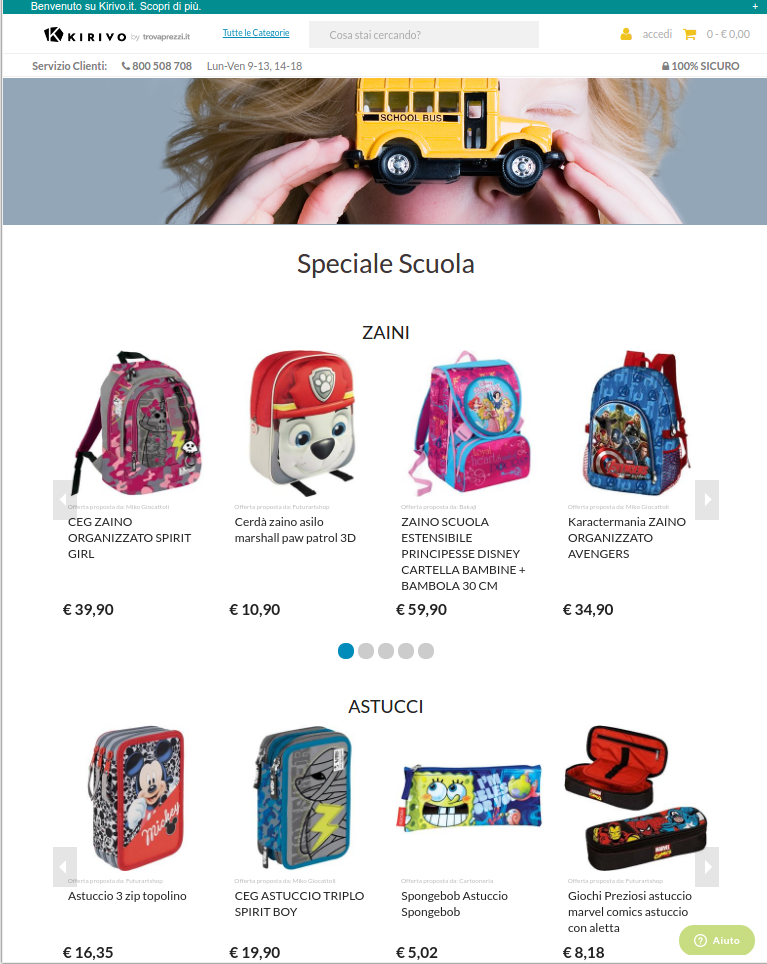
\includegraphics[width=\textwidth]{figure/speciale.png}
  \caption{Il contenuto di uno speciale.}
  \label{fig:spcial}
\end{figure}